\section{Results and discussion}

\subsection{Benchmarks and verification} \label{sec:res_benchmarks}

\subsubsection{Benchmarks for the brute force approach, no repulsion or Jastrow factor} \label{sec:res_N2N6_norep}
Table \ref{tab:N2_norep} shows the results from the brute force simulation of the two electron - no repulsion case. 
A plot of the results is shown in figure \ref{fig:N2_norep}. 

\begin{table}[h!]
	\centering 
	\begin{tabular}{l @{ } l @{ } l @{ } l @{ } l @{ } l @{ } l @{ } l @{ } l @{ } l @{ } l @{ } l @{ } l @{ } l @{ } l @{ } l @{ } l @{ } l}
		\toprule
		$\alpha~~~~$ & $0.0~~~~$ & $0.05~~~~$ & $0.1~~~~$ & $0.15~~~~$  & $0.2~~~~$ & $0.25~~~~$ & $0.3~~~~$ & $0.35~~~~$ & $0.40~~~~$ & $0.45~~~~$  \\
		\shaderow $E [\Jn] $ & 1.1e5 & 19.96 & 10.03 & 6.77 & 5.17 & 4.23 & 3.61 & 3.19 & 2.89 & 2.66  \\ 
		$\textrm{Variance} [\Jn^2] ~~$ & 7.4e9 & 2.0e2 & 4.8e1 & 2.0e1 & 1.1e1 & 7.0e0 & 4.5e0 & 3.1e0 & 2.2e0 & 1.5e0  \\ 
		\midrule
		$\alpha~~$ & $0.5~~$ & $0.55~~$ & $0.6 ~~$  & $0.65 ~~$ & $0.7~~$ &  $0.75~~$ & $0.8~~$ & $0.85~~$  & $0.9~~$ & $0.95~~$ \\
		\shaderow $E [\Jn] $  & 2.49 & 2.36 & 2.26 & 2.18 & 2.12 & 2.08 & 2.047 & 2.024 & 2.0096 & 2.002 \\ 
		$\textrm{Variance} [\Jn^2]$  
		& 1.1e0 & 7.9e-1 & 5.6e-1 & 3.9e-1 & 2.6e-1 & 1.7e-1 & 1.0e-1 & 5.3e-2 & 2.6e-2 & 5.2e-3 \\
		\midrule
		$\alpha~~$ & $1.0~~$ & $1.05~~$ & $1.1~~$ & $1.15~~$  & $1.2~~$ & $1.25~~$ & $1.3 ~~$  & $1.35 ~~$ & $1.4 ~~$ & $1.45~~$ \\ 
		\shaderow $E [\Jn] $ & 2 & 2.0029 & 2.010 & 2.021 & 2.035 & 2.05 & 2.07 & 2.09 & 2.12 & 2.14 \\ 
		$\textrm{Variance} [\Jn^2]$ & 3.3e-13 & 4.7e-3 & 1.8e-2 & 3.9e-2 & 6.7e-2 & 1.0e-1 & 1.4e-1 & 1.8e-1 & 2.3e-1 & 2.9e-1 \\ 
	\bottomrule
	\end{tabular}
	\caption{Table showing the results from the brute force VMC simulation of the expectation value of the local energy $\langle E_L \rangle$ for $\alpha$ between $0$ and $1.45$ in the 2-electron case with no repulsion or Jastrow factor. 
	The results show a minimum for the energy at $\alpha = 1$, as expected, and the variance at this point is so small that we expect it to be an eigenstate of the system.
	Units: see section \ref{sec:theory_natural_units}.}
	\label{tab:N2_norep}
\end{table}


\begin{figure}[h!]
	\centering 	
	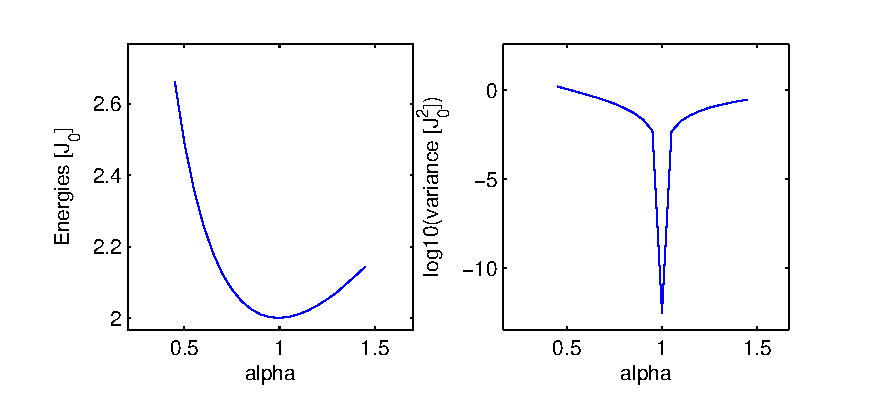
\includegraphics[width=\textwidth]{results/N2_norep.eps}
	\caption{Plot of the values given in table \ref{tab:N2_norep}, the brute force VMC simulation of the two-electron no repulsion or Jastrow factor case. 
	Some of the first values of $\alpha$ has been omitted to make the graph more informative.}
	\label{fig:N2_norep}
\end{figure}

The figure shows exactly what we would expect from the discussion of section \ref{sec:motivation}. 
The energy is always larger than $2 \Jn$ and takes this value only when $\alpha = 1$. 
We also see a huge drop in the variance just as we reach $\alpha = 1$ which indicates that this is indeed an eigenstate of the system.
What little is rest of the variance at $\alpha=1$ can be due to numerical errors in the calculation of the laplacians. 
This has in retrospect been verified to be true by using the analytical expression for the local energy. 

Table \ref{tab:N6_N12_norep} shows the result from the $N=6$ and $N=12$ electrons case with no repulsion using the brute force approach with numerical evaluation of the local energy.

\begin{table}[h!]
	\centering 
	\begin{tabular}{l @{}l @{ } l @{ } l @{ } l @{ } l @{ } l}
		\toprule
		\multirow{3}{*}{N=6}$~~\quad ~~$ & $\alpha~~~~$ & $0.9~~~~~~~~~~~~~$ & $0.95~~~~~~~~~~~~~$ & $1~~~~~~~~~~~~~$ & $0.105~~~~~~~~~~~~~$  & $0.11$ \\
		 & $E [\Jn]$ & 15.0803 & 15.0850 & 15 & 15.0184 & 15.0708\\ 
		 & $\textrm{Variance} [\Jn^2] ~~$ & 2.49e-1 & 5.89e-2 & 2.56e-13 & 2.36e-2 & 2.05e-1\\ 
		\midrule
		\multirow{3}{*}{N=12} & $\alpha~~~~$ & $0.9~~~~$ & $0.95~~~~$ & $1~~~~$ & $0.105~~~~$  & $0.11$ \\
		& $E [\Jn] $ & 42.2114 & 42.0497 & 42 & 42.0563 & 42.1937 \\ 
		& $\textrm{Variance} [\Jn^2] ~~$ & 6.92e-1 & 1.66e-1 & 1.72e-10 & 1.48e-1 & 5.69e-1\\ 
		\bottomrule
	\end{tabular}
	\caption{The results from calculating the expectation value of the local energy and its variance.
			We see that the code works for the $N=6$ and $N=12$ case because we are producing the expected results, $E_6 = 15 \Jn$ and $E_{12} = 42 \Jn$ ($\omega = 1.5 \Hzn$). 
			The variance at $\alpha=1$ is so small that we probably have the exact wave function.}
	\label{tab:N6_N12_norep}
\end{table}

The table shows that we are able to produce the results we anticipated.
Once again, we see a little variance at $\alpha=1$ which is probably due the numerical evaluation of the local energy. 
The table also showns that the code has implemented the oscillator frequency $\omega$ correctly. 










\subsubsection{Benchmark for the brute force approach, with repulsion and Jastrow factor}\label{sec:res_N2_rep}

A plot of the energies and $log_{10}$ of the variances after the investigation into finding the ground state energy for the $N=2$ electrons, with repulsion and Jastrow factor,
is shown in figure \ref{fig:N2_rep}.

\begin{figure}[h!]
	\centering
	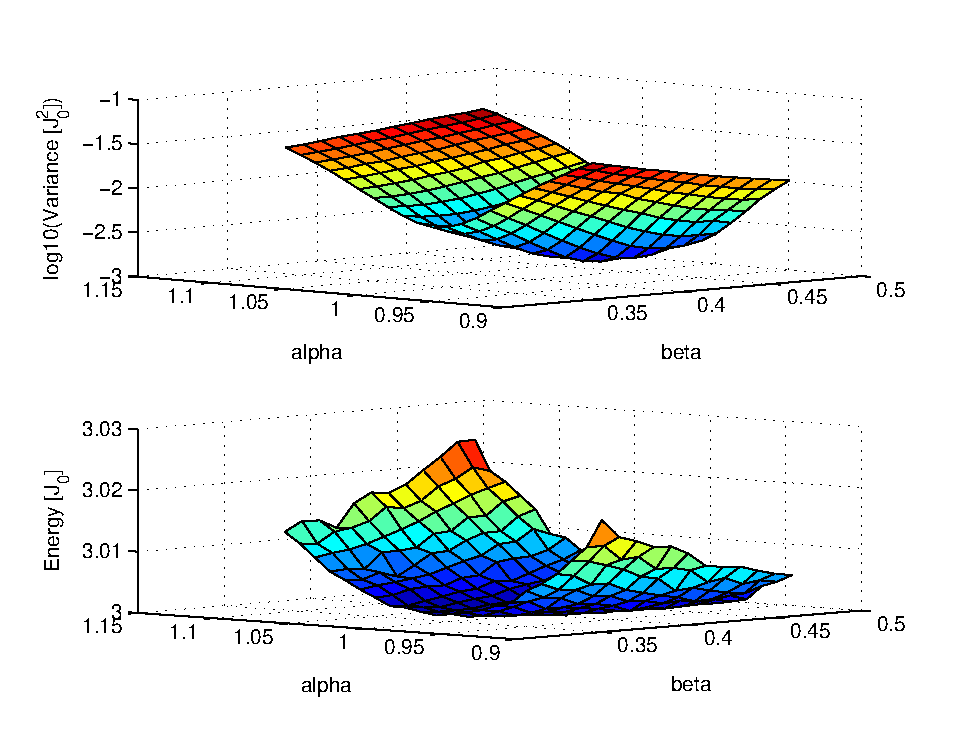
\includegraphics[width=\textwidth]{results/N2_rep.eps}
	\caption{Plot of the expectations of the local energy and $log_{10}$ of variances after the VMC simulations with two electrons, with repulsion and Jastrow factor. 
	Each point was based on $10^6$ simulations. 
	The figure gives an overview of how the energies vary as function of $\alpha$ and $\beta$.
	The lowest energy $E= 3.00022 \Jn$ where $\alpha = 0.98$ and $\beta = 0.42$.}
	\label{fig:N2_rep}
\end{figure}

It is impossible to see from the figure what is the lowest energy, but manipulating the figure in matlab revealed the smallest test state energy, which is given in table \ref{tab:N2_rep}.

\begin{table}[h!]
		\centering 
	\begin{tabular}{l}
		\toprule
		The lowest energy $E=3.00022 \Jn$ and $\textrm{Variance} = 0.001568 \Jn^2$ at $\alpha = 0.98$ and $\beta = 0.42$. \\
		\bottomrule
	\end{tabular}
	\caption{The lowest energy found from the VMC study of the two electron case with repulsion and Jastrow factor.}
	\label{tab:N2_rep}
\end{table}

The lowest energy was also found in the region where the variance was lowest. 
It seems thus that the value obtained in this VMC calculation is very close to the real lowest eigenstate. 
Very close, however, does not mean that we have found \textit{the} eigenstate. 
As we saw in the previous section, when we hit the exact eigenstate, the variance dropped rapidly to sizes in order of magnitude $10^{-12}-10^{-13}$ which was not the case here. 



\subsubsection{Comparison of different methods}\label{sec:res_methods_E}

The results from calculating $\langle E \rangle$ for the different method combinations and problem/wave function parameters are shown in table \ref{tab:methods_E}.

\begin{table}[h!]
	\centering
	\begin{tabular}{l @{ } l @{ } l @{ } l @{ } l @{ } l @{ } l  @{ } l  @{ } l  @{ } l }
	\toprule
	  & \multicolumn{3}{c}{Problem and wave function parameters} \\
	 Method parameters $~~~~$ & (2, 1, Jf, 0, 1, Ef) $~$ & (12, 0.5, Jf, 0, 1.5, En) $~$ & (6, 0.82, Jo, 0.22, 3, En)  \\
	\midrule
	(BF, NLE) & 				(2.000, 6e-13)		&		(92.10, 67.54)		&		(54.74, 28.11)			\\
	\shaderow (BF, ALE)	 &		(2.000, 0)			&		(92.18, 161.4)		&		(54.72, 28.19)		\\
	(IS, NLE, NQF) & 			(2.000, 6e-14)		&		(92.15, 66.43)		&		(54.72, 27.33)				 \\
	\shaderow(IS, NLE, AQF) &	(2.000, 1e-13) 		&		(92.06, 54.49)		&		(54.72, 27.32)						\\
	(IS, ALE, NQF) &			(2.000, 0)			&		(92.13, 143.2)		&		(54.76, 27.35)					\\
	\shaderow (IS, ALE, AQF) &	(2.000, 0) 			&		(92.12, 76.24)		&		(54.74, 27.44)	 				\\
	\bottomrule
	\end{tabular}
	\caption{A table of the expectation value and variance (Energy$[\Jn]$, Variance$[\Jn^2]$) of the local energy obtained with different problem/wave function parameters (N,$\alpha$, Jn/Jf, $\beta$, $\omega$, En/Ef). For explanation of abbreviations, see section \ref{sec:exp_methods_E}.
	For all trials, $10^6$ VMC calculations were performed and for the importance sampling methods, a time step of $\delta t = 0.1$ was used.
	The table shows that the different methods produce the same result.}
	\label{tab:methods_E}
\end{table}

These are very strong results. 
Firstly, we have verified the numerical brute force method against known benchmarks and seen that they are correct,
thus, it seems that the other methods are working properly as well!
Secondly, the different methods used very different ways to obtain the results. 
That the results are almost the same is a strong indication that all the methods are doing the same thing and functionning correctly. 















\subsection{Optimization and differences} \label{sec:res_opt_and_diff}

\subsubsection{Test cases} \label{sec:res_test_cases}

The results from finding the optimal parameters for $\alpha$ and $\beta$ for the different test cases are given in table \ref{tab:test_cases}.

\begin{table}[h!]
	\centering 
	\begin{tabular}{c  c c  c  c  c  c }
	\toprule
	 Test cases: 			& \multicolumn{2}{c}{$\omega=0.01 \Hzn$} & \multicolumn{2}{c}{$\omega=0.10 \Hzn$} & \multicolumn{2}{c}{$\omega=0.28 \Hzn$} \\
	 Optimal parameters  & No Jast. & 	Jast. & 	No Jast. & 	Jast &		No Jast. & 	Jast. \\
	 \midrule
	 $\alpha$& 				0.30 & 		0.91 & 		0.56	&	0.93	&	0.60 & 		0.96 		\\
	 $\beta$ & 				- & 		0.07 & 		-		&	0.18	&	- & 		0.26 	\\
	 \midrule
	 Energy$[\Jn]$ &		1.03e-1 &	7.40e-2 &	5.25e-1	&	4.41e-1	&	1.14  &		1.02 \\
	 Variance$[\Jn^2]$ &	1.12e-2 &	1.48e-5	& 	1.53e-1	&	2.76e-4	&	9.43e-1 & 	7.05e-4 	\\
	\bottomrule
	\toprule
	 Test cases: 			& \multicolumn{2}{c}{$\omega=0.50 \Hzn$} & \multicolumn{2}{c}{$\omega=0.75 \Hzn$} & \multicolumn{2}{c}{$\omega=1 \Hzn$} \\
	 Optimal parameters  & No Jast. & 	Jast. & 	No Jast. & 	Jast. & 	No Jast. & Jast. \\
	 \midrule
	 $\alpha$& 				0.70 & 		0.97 & 		0.74 & 		0.98 	& 	0.72	& 	0.97 	\\
	 $\beta$ & 				- & 		0.32 & 		- & 		0.38 & 		-  		& 	0.42 	\\
	 \midrule
	 Energy$[\Jn]$  & 		1.80 &		1.66 &		2.50  &		2.34 & 		3.15 & 		3.00	\\
	 Variance$[\Jn^2]$ & 	1.25 &		1.01e-3	& 	1.69 & 		1.35e-3 & 	2.03 & 		2.7e-3 	\\
	 \bottomrule
	\end{tabular}
	\caption{The optimal parameters with and without Jastrow factor (Jast.) for different oscillator
			 potentials.
			 Results were produced by calculating the energy for every $\alpha$ and $\beta$ in the interval $[0,1.2]$ with 	a step length of $0.01$ and $10^5$ MC simulation.
			 The estimates with the Jastrow factor are better than those without.}
	\label{tab:test_cases}
\end{table}

The result for $\omega =1 \Hzn$ with Jastrow factor is almost in perfect agreement with what was found in section \ref{sec:res_N2_rep}, even though the method of finding the optimal parameters was different. 
This indicates that the results obtained are reliable even though only $10^5$ simulations were performed. For the purpose of this section, they are probably good enough. 

Another approach to get these parameters would be to do a similar approach as in section \ref{sec:res_N2_rep} for each case. 
This proved to be too time-consuming, and an automated approach such as the one used here could be run overnight, which was done here. 
For a further discussion on code efficiency and time constraints, see section \ref{sec:ce_tc}.



\subsubsection{Jastrow factor}\label{sec:res_jastrow}

The relative change in energy (i.e. correlation) due to the Jastrow factor for the test cases is given in table \ref{tab:correlations_jastrow}.

\begin{table}[h!]
	\centering
	\begin{tabular}{ccccccc}
	\toprule
	$\omega$	& 0.01 & 0.10 & 0.28 & 0.50 & 0.75 & 1 \\
	\midrule
	Correlation $C = \frac{E_{NJ} - E_{J}}{E_{NJ}}$ & 0.282 & 0.160 & 0.105 & 0.078 & 0.064 & 0.048 \\
	\bottomrule
	\end{tabular}
	\caption{The correlation introduced by the Jastrow factor for the optimal parameters $\alpha$ and $\beta$ as a function of $\omega$. 
	We see that the correlation factor is less important for high oscillator potentials.
	"NJ" means no Jastrow factor and "J" means with Jastrow factor.}
	\label{tab:correlations_jastrow}
\end{table}

A plot of the correlations in table \ref{tab:correlations_jastrow} is given in figure \ref{fig:correlations_jastrow}. 

\begin{figure}[h!]
	\centering 
	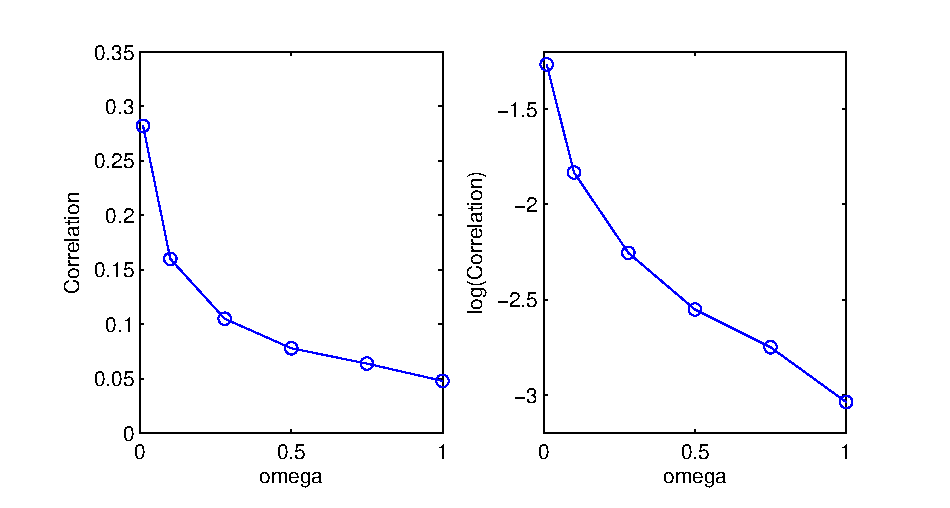
\includegraphics[width=\textwidth]{results/correlations_jastrow.eps}
	\caption{Plot of the correlation introduced by the Jastrow factor for the optimal parameters $\alpha$ and $\beta$ as a function of $\omega$. 
	From the left figure one may suspect a curve of the shape $C = C_0 \exp(-k\omega)$ but the right hand plot of $\textrm{ln}(C)$ against $\omega$ does not look very linear which weakens this hypothesis.}
	\label{fig:correlations_jastrow}
\end{figure}

Our first observation is that the Jastrow factor does indeed better our estimation of the ground state energy. 
We already knew from section \ref{sec:res_N2_rep} that the including the Jastrow factor gave us a very good estimate of the ground state energy when $\omega = 1$, and from table \ref{tab:test_cases}  we see that the ratio between variance and energy estimate is small and almost constant ($\sim 5 \times 10^{-4}$) in the case with the Jastrow factor as opposed to the case without the Jastrow factor. 

Our second observation from both the table and the figure is that the correlations get smaller as the oscillator frequency increases. 
This is a counter-intuitive result.
Normally one would expect the repulsion between the electrons to be more important the closer together the electrons are.
One can try to explain the phenomenon by looking at another, equivalent expression of the expectation value of the local energy.

\eqs
\langle E_L \rangle = \langle K \rangle + \langle V_{HO} \rangle + \langle V_{ER} \rangle 
\eqf

Where $\langle K \rangle$ is the expectation value of the kinetic energy, $\langle V_{HO} \rangle$ that of the harmonic oscillator potential and $\langle V_{ER} \rangle$ that of the electron repulsion potential.
It seems that as $\omega$ increases, all these values increase, but the relative size of $\langle V_{ER} \rangle $ decreases, so for large $\omega$, the role played by $\langle V_{ER} \rangle$ gets smaller and smaller.

From the left hand plot in the figure, one might suspect that the correlation decreases exponentially as a function of $\omega$. 
To test this, a plot of $\textrm{ln}(C)$ against $\omega$ has been included in the right hand plot. 
If this hypothesis was true, the result should be a straight line, but alas, it is not. 
It is therefore probably some other rule governing the relation between $C$ and $\omega$. 





\subsubsection{Importance sampling} \label{sec:res_importance_sampling}

The results from evaluation of $\langle E_L \rangle$ as a function of Monte Carlo simulations and time steps $\delta t$ are given in table \ref{tab:importance_sampling} and figure \ref{fig:importance_sampling}.

\begin{table}[h!]
	\centering 
	\begin{tabular}{l @{ } l @{ } l @{ } l @{ } l @{ } l @{ } l @{ } l @{ } l @{ } l }
	\toprule
	\multicolumn{9}{l}{Energies obtained with the brute force method} \\
	MCS \textbackslash  $\delta t = \quad$ & $10^{-6}~~~$ & $10^{-5}~~~$  & $10^{-4}~~~$  & $10^{-3} ~~~$  & $ 10^{-2} ~~~$ & $ 10^{-1} ~~~$  & $ 1 \qquad $  & $ 10 ~~~~$  & $ 10^{2}$ \\
	\midrule
	$10^3$ & 3.26 &  3.21 & 3.16 & 3.24 &  3.35 &  3.29 & 3.36 &  3.11 &  3.25\\
	\shaderow $10^4$ &  3.21 &   3.22 &    3.22 &   3.27 &  3.25 &  3.26 & 3.24 &   3.22 &  3.26 \\
	$10^5$ & 3.23 &    3.24 &   3.21 &  3.22 &  3.24 &  3.23 & 3.24 &   3.24 &  3.23 \\
	\shaderow $10^6$ & 3.23 &   3.23 &   3.23 &  3.23 &   3.24 &  3.24 & 3.24 &   3.24 &  3.24 \\
	\bottomrule
	\toprule
	\multicolumn{9}{l}{Energies obtained with importance sampling} \\
	MCS \textbackslash  $\delta t = \quad$ & $10^{-6}~~~$ & $10^{-5}~~~$  & $10^{-4}~~~$  & $10^{-3} ~~~$  & $ 10^{-2} ~~~$ & $ 10^{-1} ~~~$  & $ 1 ~~~~$  & $ 10 ~~~~$  & $ 10^{2}$ \\
	\midrule
	$10^3$ & 7.78 &   2.13 &   4.49 &  4.01 &  3.25 &  3.21 &   3.28 &  3.23 &  2.86 \\
	\shaderow $10^4$ &  3.95 &   2.74 &   2.42 &   3.19 &  3.33 &  3.29 &   3.21 &   3.18 &   4.02 \\
	$10^5$ & 2.46 &  3.58 &   3.22 &   3.26 &  3.21 &   3.23 &  3.20 &   3.07 &   5.40 \\
	\shaderow $10^6$ & 3.99 &   3.41 &  3.13 &  3.22 &  3.24 &  3.22 &  3.20 &  4.60 &  2.60 \\
	\bottomrule
	\end{tabular}
	\caption{Energies obtained with the brute force method and the importance sampling method as function of number of  		Monte Carlo simulations (MCS) and time step $\delta t$ (in$\sn$). 
			Brute force energy estimates do naturally not vary with $\delta t$ since the latter do not play a role in the brute force method. 
			The different energies obtained with the brute force method are thus only repetitions of the same simulation.
			Importance sampling seem to be stable around $\delta t = 10^{-2}\sn$.}
	\label{tab:importance_sampling}
\end{table}


\begin{figure}[h!]
	\centering 
	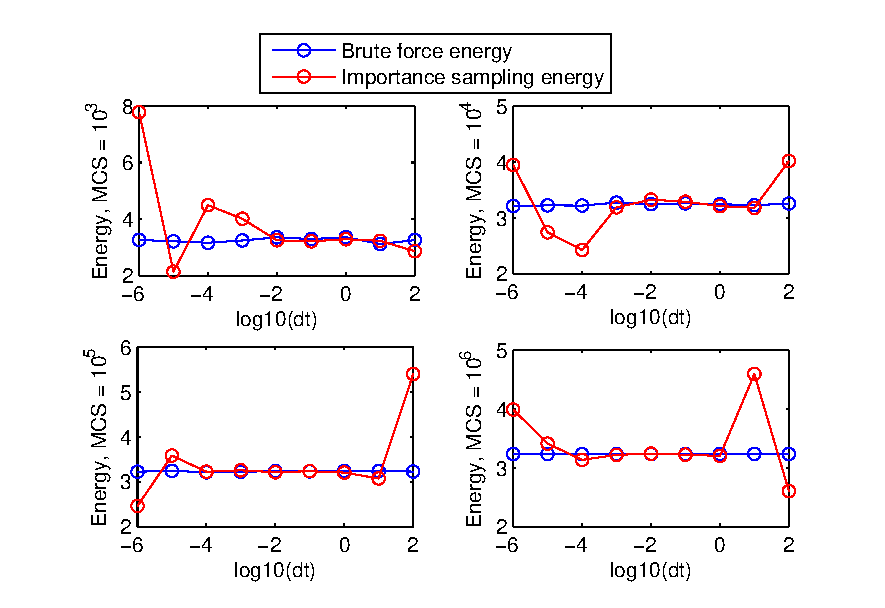
\includegraphics[width=\textwidth]{results/importance_sampling.eps}
	\caption{Plot of the energies evaluated by the brute force method and the metropolis method as a function of number of Monte Carlo simulations (MCS) and time step $\delta t$.
	The method seems stable around $\delta t = 10^{-2} \sn$ and interval of $\delta t$'s in which the method seems to be stable increases with the number of Monte Carlo simulations.}
	\label{fig:importance_sampling}
\end{figure}

We see from the results that the reliability of using importance sampling depends greatly on the time step chosen. 
The results seem to coincide with the brute force method when $\delta t \approx 10^{-2} - 10^{-1} \sn$.
This is natural because if $\delta t$ is too small, the steps in the metropolis algorithm does also become very small. 
It then takes a large number of Monte Carlo simulations for the metropolis walker to move across a representative  selection of points. 
This is illustrated by the figure by noticing that as the number of Monte Carlo simulations gets larger, a greater range of $\delta t$'s converges to the proper solution. 
When $\delta t$ gets too large, the step length gets too large and we have little control over how the energy estimates will behave. 

The energy estimates by the brute force method does not vary with $\delta t$. 
This is natural because $\delta t$ plays no role in the evaluation of $\langle E_L \rangle$ with the brute force method. 
The different energies obtained for different $\delta t$'s are thus just repetitions of the same measurement, and serve only as a illustration of the uncertainty in the evaluation of $\langle E_L \rangle$. 
For the purposes of this project, it seems that the brute force method serves as a stable and reliable method for calculating $\langle E_L \rangle$ with good precision only with $10^3$ Monte Carlo simulations. 
For more complex problems, it may be that importance sampling, with its foundation in the physical system, attributes to greater precision in producing results, but for the problems discussed here, it seems that it only introduces a new uncertainty in whether the time step $\delta t$ has been chosen correctly. 

The acceptance rate of the importance sampling method as a function of the time step $\delta t$ is given in table \ref{tab:IS_accept}.

\begin{table}[h!]
	\centering 
	\begin{tabular}{l l l l l l l l l l l l  l l l l }
	\toprule
	$\delta t [\sn]$ & $10^{-6}$ & $10^{-5}$  & $10^{-4}$  & $10^{-3} $  & $ 10^{-2} $ & $ 10^{-1} $  & $ 1 $  & $ 10 $  & $ 10^{2}$\\
	\midrule
	AR: & 1 & 1 & 1 & 0.99999 & 0.9997 & 0.991 & 0.769 & 0.00136 & 0 \\
	\bottomrule
	\end{tabular}
	\caption{The acceptance rate (AR) when using the metropolis algorithm as a function of $\delta t$. 
			For a reasonably low time step, the acceptance rate is nearly at $100 \%$, whereas it falls quickly down to zero once the timestep gets to big.}
	\label{tab:IS_accept}
\end{table}

From the table, we see what we expected. 
For a small enough time step, the acceptance rate is nearly at $1$ and as the time step gets too large, it falls to $0$. 
Since we found the proper interval for $\delta t$ to be between $10^{-2}$ and $10^{-1}$, we can safely say that using the importance sampling method greatly increases the acceptance rate. 







\subsubsection{Timely differences between methods} \label{sec:res_timely_diff}

Table \ref{tab:res_times} shows the time used by the different methods for the two different test cases.
A plot of the times used are given in figure \ref{fig:res_times}. 

\begin{table}[h!]
	\centering 
	\begin{tabular}{l @{ } l @{ } l @{ } l @{ } l @{ } l @{ } l @{ } l @{ } l }
	\toprule
	\multicolumn{9}{l}{2 electrons with repulsion and Jastrow factor, $\alpha = 0.77$ and $\beta = 0.22$.} \\
	Method \textbackslash $MCS = ~~~$ & $10^3~~~~~~~$ & $3\times 10^3~~$ & $10^4~~~~~~~$ & $3\times 10^4~~$ & $10^5~~~~~~~$ & $3\times 10^5~~$ & $10^6~~~~$ & $3\times 10^6$ \\
	\midrule
	(BF, NLE) & 1.87e-2 & 4.11e-2 & 1.36e-1 & 2.59e-1 & 7.14e-1 & 2.10 & 6.53 & 19.5 \\
	\shaderow (BF,ALE) & 9.75e-3 & 2.86e-2 & 9.45e-2 & 1.43e-1 & 3.08e-1 & 7.80e-1 & 2.44 & 7.39 \\
	(IS, NLE, NQF) & 1.81e-2 & 5.52e-2 & 1.82e-1 & 5.46e-1 & 1.82 & 5.45 & 18.1 & 54.4 \\
	\shaderow (IS, NLE, AQF) & 1.30e-2 & 3.88e-2 & 1.30e-1 & 3.89e-1 & 1.29 & 3.88 & 12.9 & 38.8 \\
	(IS, ALE, NQF) & 1.12e-2 & 3.22e-2 & 1.08e-1 & 3.19e-1 & 1.06 & 3.18 & 10.7 & 31.9 \\
	\shaderow (IS, ALE, AQF) & 5.30e-3 & 1.59e-2 & 5.28e-2 & 1.59e-1 & 5.30e-1 & 1.59 & 5.30 & 15.9 \\
	\bottomrule
	\toprule
	\multicolumn{9}{l}{6 electrons with repulsion and Jastrow factor, $\alpha = 0.49$ and $\beta = 0.39$.} \\
	Method \textbackslash $MCS = ~~~$ & $10^3~~~~~~~$ & $3\times 10^3~~$ & $10^4~~~~~~~$ & $3\times 10^4~~$ & $10^5~~~~~~~$ & $3\times 10^5~~$ & $10^6~~~~$ & $3\times 10^6$ \\
	\midrule
	(BF, NLE) &  1.44e-1 & 3.85e-1 & 1.25 & 3.06 & 10.0 & 28.4 & 94.3 & 283 \\
	\shaderow (BF,ALE) &  4.75e-2 & 1.47e-1 & 4.89e-1 & 7.79e-1 & 1.86 & 4.80 & 14.8 & 46.2 \\
	(IS, NLE, NQF) & 2.91e-1 & 8.73e-1 & 2.91 & 8.71 & 29.1 & 87.1 & 290 & 870 \\
	\shaderow (IS, NLE, AQF) & 1.91e-1 & 5.71e-1 & 1.90 & 5.70 & 19.0 & 56.9 & 190 & 570 \\
	(IS, ALE, NQF) & 1.40e-1 & 4.20e-1 & 1.40 & 4.19 & 14.0 & 42.0 & 140 & 420 \\
	\shaderow (IS, ALE, AQF) & 3.97e-2 & 1.20e-1 & 3.98e-1 & 1.19 & 4.05 & 11.9 & 39.7 & 120 \\
	\bottomrule
	\end{tabular}
	\caption{Time (in seconds) used by the different methods as a function of Monte Carlo simulations (MCS).
			See section \ref{sec:exp_methods_E} for method abbreviations.
			The CPU-time spent using analytical expression is dramatically reduced. }
	\label{tab:res_times}
\end{table}


\begin{figure}[h!]
	\centering 
	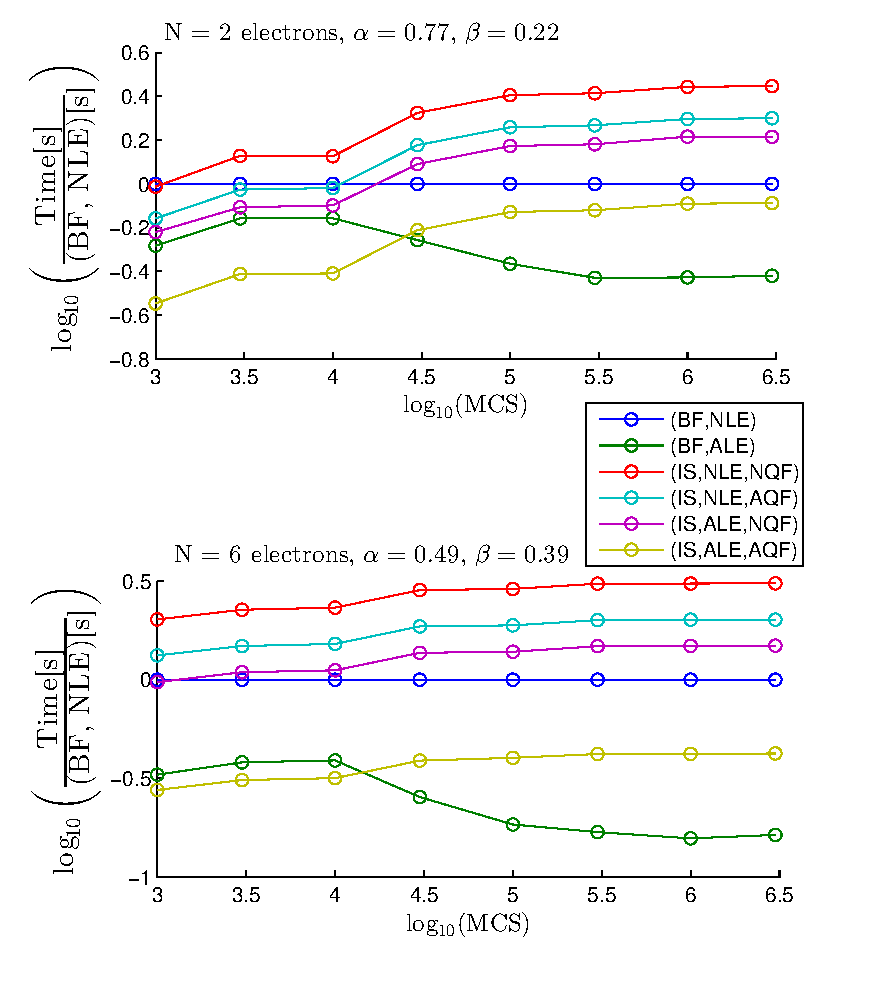
\includegraphics[width=\textwidth]{results/times.eps}
	\caption{$\textrm{log}_{10}$ of the time (in seconds) used by the different methods relative to the brute force, numerical local energy method as a function of $\textrm{log}_{10}$ of Monte Carlo simulations.
	The most efficent method for large $MCS$ is the brute force approach with numerical expressions for the local energy. }
	\label{fig:res_times}
\end{figure}

From the result we see that the relative difference in the time spent by the different methods stabilize after $\sim 10^5$ Monte Carlo simulations. 
After this point, the brute force metropolis algorithm with the analytical expression for the local energy is the most time efficient method, both for $N=2$ and $N=6$.
For the $N=6$ case, the latter method uses in fact almost as little as $1/20$ of the time the slowest method (Importance sampling, numerical expressions) needs. 
To begin with, at $10^3$ Monte Carlo simulations, importance sampling with analytical expressions is the fastest method.
This is because the brute force method needs to run a couple of simulations without sampling to begin with in order to achieve the wanted acceptance rate of $0.5$ whereas the importance sampling method can begin straight away sampling points. 
But as the number of Monte Carlo simulations increase however, this head start gets relatively smaller. 

We also see that whenever analytical expressions is used instead of numerical ones, the efficiency is increased. 
From the figure we see that when using importance sampling, the implementation of the analytical local energy produces a greater increase in efficiency than implementing analytical expressions of the quantum force.
And only when implementing both analytical expressions for the local energy \textit{and} the quantum force is the importance sampling method superior to the brute force, numerical local energy method. 



\clearpage

















\subsubsection{Discussion: code efficiency and time constraints}\label{sec:ce_tc}

The code upon which this project is built has a lot of potential for improvement. 
Lots of the methods developed in this project has been programmed to the point at which the worked, and time constraints have cut short further improvements with regards to code efficacy.
Examples of things that could have improved general code efficacy are things as 

\begin{itemize}
	\item \textbf{Reducing the amount of times a variable is calculated}:
	Although this aspect have been in the back of my mind while programming, I'm sure that a thorough review of the code would reveal a lot of potential. 
	\item \textbf{Avoiding too many divisions}: 
	Divisions in a computer is normally more slow than multiplication\footnote{Source: \href{http://streamcomputing.eu/blog/2012-07-16/how-expensive-is-an-operation-on-a-cpu/}{http://streamcomputing.eu/}}. Replacing recurrent divisions by clever multiplication might have improved code efficiency.
	\item \textbf{Reduce usage of complicated functions such as $\sin$, $\exp$ etc}:
	Although I have put some thought into this while designing the code, there are probably some places where a lot of CPU time could be saved. 
\end{itemize}

There are also things more specific to this project that could have improved code efficiency. Examples are

\begin{itemize}
	\item \textbf{More efficient ratio calculations}:
	In the Metropolis algorithm used in this project, a ratio of the wave functions squared was evaluated. 
	But since we only move \textit{one} particle at a time, a lot of the so-called \textit{co-factors} in the Slater determinant cancel\footnote{Page 81, \cite{master}.} and reduces the number of expressions we need to calculate. If this were adjusted for, I think a lot of computational time could have been saved.
	\item \textbf{Re-usage of some expressions}:
	In the calculation of the analytical local energy, the terms needed for the analytical quantum force was also calculated. One could implement this into the code so that if the analytical expression for the local energy was evaluated \textit{and} importance sampling was used with analytical quantum force, the expressions would reused and not calculated twice. 
	There might also be other such examples of expressions which are evaluated multiple times in this code.
	\item \textbf{Better usage of OpenMP parallelization}:
	An interesting question is how much time it takes for OpenMP to communicate between the different threads.
	If this would prove itself a significant issue, then a better implementation of parallelization could have saved some time. 
\end{itemize}

Finally there is the matter of method for finding the optimal parameters $\alpha$ and $\beta$. 
In this project, I used a very brute force method for which I could only spare $10^5$ MC simulations for each energy in order for the process not to take weeks. 
A better algorithm for finding the optimal $\alpha$ and $\beta$ was not in the scope of this project, but I believe it could seriously improve the efficacy of the process.

But all things considered, I am happy to have paid the price of a slow running code in exchange for having been able to implement lots of different methods for solving the problems discussed in this project. 
Even though the weak efficiency is probably affecting the precision of the result in the next section in a negative manner, the results are still correct within a certain margin of error.
Also, the code is not going anywhere, so if I later want to improve upon it and implement better algorithms for finding $\alpha$ and $\beta$ I am free to do so, even I don't have time to do so before the deadline of this project. 









\subsection{Applications}

\subsubsection{Properties of the approximated wave functions} \label{sec:res_properties}

The interesting properties of the approximated wave functions and the optimal variables for the six new test cases are given in table \ref{tab:interesting_quantitities}. 

\begin{table}[h!]
	\centering 
	\begin{tabular}{l@{ } l@{ } l@{ } l@{ } l@{ } l@{ } l}
		\toprule
		$N=2$ electrons & $\omega = 0.01 \quad $ &  $\omega = 0.10 \quad $ & $\omega =0.28 \quad $  & $\omega = 0.5 \quad $ & $\omega = 0.75 \quad $ & $\omega = 1$ \\
		\midrule
		Energy $\langle H \rangle$  & 	7.40e-2 & 4.41e-1 & 1.02  & 1.66 & 2.34 & 3.00\\
		\shaderow Variance $[\Jn^2]$  &	1.09e-5 & 2.74e-4 & 6.86e-4 & 1.03e-3  & 1.32e-3 & 1.78e-3 \\
		Average distance $[\mn]$& 	29.4 & 6.72 & 3.53 & 2.47 & 1.92 & 1.63 \\
		\shaderow Potential Energy $\langle V \rangle \quad $  & 6.43e-2 & 3.5e-1 & 7.71e-1 & 1.22 & 1.67 & 2.12 \\ 
		Kinetic Energy $\langle T \rangle$  &  9.74e-3 & 9.09e-2 & 2.51e-1  & 4.44e-1 & 6.70e-1 & 8.81e-1 \\
		\bottomrule
		\toprule
		$N=6$ electrons & $\omega = 0.01$ &  $\omega = 0.10$ & $\omega =0.28$ & $\omega = 0.5$ & $\omega = 0.75$ & $\omega = 1$ \\
		\midrule
		Optimal $\alpha$ & 0.61 & 0.83 & 0.88 & 0.93 & 0.9 & 0.93 \\
		\shaderow Optimal $\beta$  & 0.10 & 0.22 & 0.33 & 0.38 & 0.5 & 0.57 \\
		Energy $\langle H \rangle$   & 6.99e-1 & 3.57 & 7.62 &  11.8 & 16.1 & 20.2 \\
		\shaderow Variance $[\Jn^2]$  & 2.98e-4 & 4.52e-3 & 1.88e-2  & 4.59e-2 & 8.42e-2 & 1.33e-1 \\
		Average distance $[\mn]$& 39.6 &	9.16 & 4.83 & 3.42 & 2.68 & 2.23 \\
		\shaderow Potential Energy $\langle V \rangle $ & 6.71e-1 &  3.24 & 6.68 & 10.1 & 13.5 & 16.6 \\ 
		Kinetic Energy $\langle T \rangle$ & 2.76e-2 &  3.30e-1 & 9.56e-1 & 1.74 & 2.6 & 3.62 \\
		\bottomrule
	\end{tabular}
	\caption{The energies and average distances between the particles for the trial wave functions 
			corresponding to the lowest expectation values of the local energy.
			The optimal wave function parameters used for the $N=2$ electrons case are given in table \ref{tab:test_cases}.
			All energies are in units$\Jn$.}
	\label{tab:interesting_quantitities}
\end{table}

First of all, we notice that the energies obtained here, with $10^7$ Monte Carlo simulations, is the same as the ones obtained in section \ref{sec:res_test_cases} with $10^5$ Monte Carlo simulations to the third digit.
Which is an indication that $10^5$ simulations to find $\alpha$ and $\beta$ was not to little. 

As we might expect, the higher the frequency of the oscillator potential, the closer the electrons are to each other.
This is because the electrons are "squeezed" together by the potential.  
A plot of the average electron distance for both $N=2$ electrons and $N=6$ electrons as a function of $\omega$ is given in figure \ref{fig:AD_electrons}.

\begin{figure}[h!]
	\centering 
	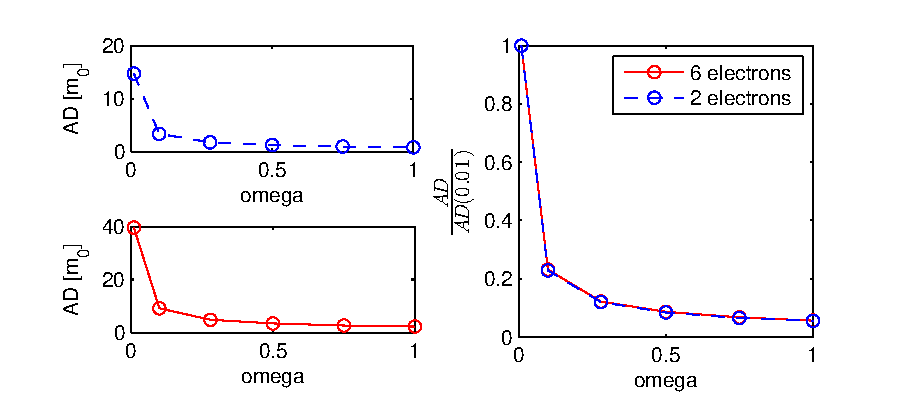
\includegraphics[width=\textwidth]{results/AD.eps}
	\caption{Plot of the average distance (AD) between the electrons for the optimal trial wave function for $N=2$ electrons and $N=6$ electrons. 
			The average distance decreases with $\omega$, as expected, when the potential "squeezes" the electrons together.
			The dependency of the average distance on $\omega$ is remarkably similar for $N=2$ electrons and the $N=6$ electrons case.}
	\label{fig:AD_electrons}
\end{figure}

From the figure we see that the shape of the average distance's dependence on $\omega$ is remarkably similar for the two cases.
A possible explanation of this fact is to consider the electrons as localized charges pushing each other away until the point where the curvature of the potential equals the repulsive pushing. 
The electrons would in this image form some sort equilateral shape which would not be dependent on the frequency of the oscillator and an increase in the oscillator would just reduce the "scale" of the pattern by a factor. 
That this "factor" is the same for the $N=2$ and the $N=6$ electron case is not obvious, but not unreasonable\footnote{I'm sure one could make some geometric argument as to why this is the case.} either.  
The fact that such a model can be applied to quantum mechanics however, is more surprising. 






\subsubsection{The virial theorem }\label{sec:res_virial}

A more detailed overview of the different expectation values of energies for the wavefunctions investigated in the previous section is given in  table \ref{tab:res_virial}.

\begin{table}[h!]
	\centering 
	\begin{tabular}{l@{ } l@{ } l@{ } l@{ } l@{ } l@{ } l}
		\toprule
		\multicolumn{7}{l}{$N=2$ electrons, with repulsion and Jastrow factor.} \\
			& $\omega = 0.01$ &  $\omega = 0.10 \quad $ & $\omega =0.28 \quad $  & $\omega = 0.5 \quad $ & $\omega = 0.75 \quad $ & $\omega = 1$ \\
		\midrule
		Harmonic Energy $\langle V_{HO} \rangle \quad$ &  2.82e-2 & 1.80e-1 & 4.24e-1 & 7.01e-1 & 9.91e-1 & 1.30 \\
		\shaderow Repulsive Energy $\langle V_{RE} \rangle$ & 3.61e-2 & 1.71e-1 & 3.48e-1 & 5.15e-1 & 6.82e-1 & 8.16e-1 \\
		Potential Energy $\langle V \rangle  \quad $ & 6.43e-2 & 3.5e-1 & 7.71e-1 & 1.22 & 1.67 & 2.12 \\
		\shaderow Kinetic Energy $\langle T \rangle$ &  9.74e-3 & 9.09e-2 & 2.51e-1  & 4.44e-1 & 6.70e-1 & 8.81e-1 \\
		\bottomrule
		\toprule
		\multicolumn{7}{l}{$N=6$ electrons, with repulsion and Jastrow factor.} \\
			 & $\omega = 0.01$ &  $\omega = 0.10$ & $\omega =0.28$ & $\omega = 0.5$ & $\omega = 0.75$ & $\omega = 1$ \\
		\midrule
		Harmonic Energy $\langle V_{HO} \rangle$  & 2.30e-1 & 1.26 & 2.81 & 4.52 & 6.31 & 7.80\\
		\shaderow Repulsive Energy $\langle V_{RE} \rangle$ & 4.41e-1 & 1.98 & 3.87 & 5.55 & 7.22 & 8.77\\
		Potential Energy $\langle V \rangle $ & 6.71e-1 &  3.24 & 6.68 & 10.1 & 13.5 & 16.6 \\ 
		\shaderow Kinetic Energy $\langle T \rangle$ & 2.76e-2 &  3.30e-1 & 9.56e-1 & 1.74 & 2.68 & 3.62 \\
		\bottomrule
		\toprule
		\multicolumn{7}{l}{$N=2$ electrons, without repulsion or Jastrow factor.} \\
			& $\omega = 0.01$ &  $\omega = 0.10 \quad $ & $\omega =0.28 \quad $  & $\omega = 0.5 \quad $ & $\omega = 0.75 \quad $ & $\omega = 1$ \\
		\midrule
		Potential Energy $\langle V \rangle  \quad $ & 9.94e-3 & 9.95e-2 & 2.78e-1 & 4.97e-1 & 7.46e-1 & 9.95e-1\\
		\shaderow Kinetic Energy $\langle T \rangle$ & 1.01e-2 & 1.01e-1 & 2.82e-2 & 5.03e-1 & 7.54e-1 & 1.01\\
		\bottomrule
		\toprule
		\multicolumn{7}{l}{$N=6$ electrons, without repulsion or Jastrow factor.} \\
			& $\omega = 0.01$ &  $\omega = 0.10 \quad $ & $\omega =0.28 \quad $  & $\omega = 0.5 \quad $ & $\omega = 0.75 \quad $ & $\omega = 1$ \\
		\midrule
		Potential Energy $\langle V \rangle  \quad $ &  5.00e-2 & 4.99e-1 & 1.40 & 2.50 & 3.74 & 4.99\\
		\shaderow Kinetic Energy $\langle T \rangle$ &  5.00e-2 & 5.00e-1 & 1.40 & 2.50 & 3.76 & 5.00\\
		\bottomrule
	\end{tabular}
	\caption{The different forms of energies (in$\Jn$) in the optimal wave functions for $N=2$ and $N=6$, with and without the Jastrow factor, as a function of $\omega$.}
	\label{tab:res_virial}
\end{table}

A plot of the ratio between the expectation value of the kinetic and the potential energy is given in figure \ref{fig:res_virial}.

\begin{figure}[h!]
	\centering 
	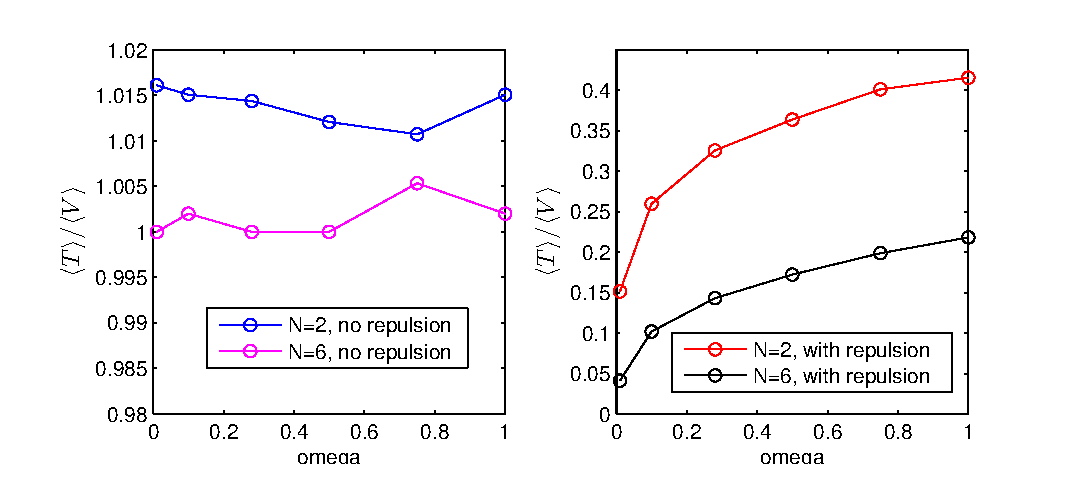
\includegraphics[width=\textwidth]{results/virial.eps}
	\caption{Plot of the ratio between the expectation value of the kinetic and potential energy as a function of $\omega$ for the optimal wavefunctions. 
	The virial theorem states that the ratio should be constant and is thus fulfilled for the no repulsion case, but not the repulsion case.}
	\label{fig:res_virial}
\end{figure}

From the figure and table, we see that the virial theorem holds very well for the no repulsion case. 
This is not surprising since as we know, we had the exact ground state. 
There does however seem to be a small favorization of kinetic energy over potential energy which is most important for the $N=2$ electron case. 
The reason for this, I believe, has to do with the sampling technique. 
The wave function is constructed in such a way that kinetic energy is most important when the distance from the origin is small an potential energy is more important for larger distances. 
This means that we may have a small over representation of the "small distance to the origin"-points in our Monte Carlo simulation. 
The reason for this might be due to the fact that our starting point \textit{is} one close to the origin. 
Another possible reason is that since we have a finite number of Monte Carlo points, some of the points \textit{very} far away from the origin will not be reached in a finite simulation, resulting in no representation of these points whereas the should have been represented to a small degree in a perfect integration. 
These explanations do not, however, explain why for the $N=6$ electron, no repulsion case, the same number of simulations seem to give better results. 
This might be due to the fact that the energy is greater with $6$ electrons, reducing the relative impact of the small misrepresentation in the sampling points. 

The other important thing to see is that the virial theorem is not furfilled for the no repulsion cases. 
Here, the ratio between $\langle T \rangle$ and $\langle V \rangle$ is dependent on $\omega$ in such a way that when $\omega$ gets smaller, the potential term is much larger than the kinetic term. 
This is a very interesting observation. 
The kinetic energy is a measure of how much movement there is in the substance (here: electrons in a trap). 
Thus, if the kinetic energy is small compared to the potential energy, this means that the electrons are very immobile and localized, in the same way that freezing water causes molecules to stay put in one place. 
Does this mean that a small oscillator potential "freezes" the electrons in place, or is this solely an artifact of the numerical method? 
If it really is another "phase", what then are the properties of this substance?
These are all fascinating questions which would be interesting to investigate another time. 
